%%%%%%%%%%%%%%%%%%%%%%%%%%%%%%%%%%%%%%%%%%%%%%%%%%%%%%%%%%%%%%%%%%%%%%%%%%%%%%%%%%%%%%%%%%%%%%%%%%
\begin{frame}
	\frametitle{Resultados para el EM}    
		\begin{overlayarea}{\textwidth}{.1\textheight}
			\vspace*{-.15cm}
			\begin{empheq}[box=\shadowbox*]{equation*}
				dy(t) = f(y(t)) dt + g(y(t)) dW_t, \quad Y_0=y_0.  \tag{EDE}
			\end{empheq}
		\end{overlayarea}
	\begin{overlayarea}{\textwidth}{.9\textheight}
		\begin{columns}
			\column{.51\textwidth}
				\begin{tcolorbox}[left=-1mm, title= Hip\'otesis:]
					\begin{enumerate}[(H1)]
						\item 
						%\structure{(H-1)}
							\scalebox{.7}{
								\textcolor{black}{
									$\forall R>0$,  $\exists \  C_R>0$
								}
							}
							\\
							\scalebox{.7}{
								\textcolor{black}{
								$	
									|f(x)-f(y)|^2 \vee |g(x)-g(y)|^2 \leq C_R|x-y|^2
								$
							}
							}
							\\
							\scalebox{.7}{
								\textcolor{black}{
								$
									\forall x,y\in \R^d 
									|x|\vee |y|\leq R.
								$
								}
							}
							\\
						\item
							%\structure{(H-2)}
							\scalebox{0.7}{
								Para alg\'un $p>2$, $\exists \  A>0$ t.q.
							}
							\scalebox{0.7}{
								\textcolor{black}{
									\textcolor<2->{red}{
										$
											\displaystyle
											\EX{\sup_{0\leq t\leq T}|\overline{Y}(t)|^p}
											\vee
											\EX{\sup_{0\leq t\leq T}|y(t)|^p} \leq A.
										$
									}
								}
							}
					\end{enumerate}	
					\tcblower
					\hspace*{.25cm}
					\only<3->{
						$	
							\overline{Y}(t):=
							Y_{\eta(t)} + (t-t_{\eta(t)}) f(Y_{\eta(t)}) 
						$	
						\\
						\hspace*{1.0cm}
						$
							+ g(Y_{\eta(t)})(W(t)-W_{\eta(t)}),\\
						$
						\hspace*{.25cm}
						$
							\eta(t):=
							k, \text{ for } t\in[t_k,t_{k+1})
						$
					}
				\end{tcolorbox}
%%								
			\column{.5\textwidth}
				\only<4->{
					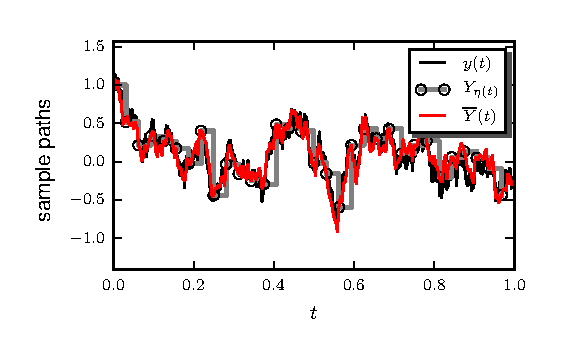
\includegraphics[width=1\linewidth]{Imagenes/HighamConvergence/ContinuousExtension.eps}
				}
				\only<5->{
					\begin{Teorema}
						EM converge
						\begin{equation*}
							\lim_{h\to 0}
							\EX{\sup_{0\leq t\leq T}|\overline{Y}(t)-y(t)|^2}=0.
						\end{equation*}
					\end{Teorema}
				}
				\only<2-3>{
					\begin{bibunit}[apalike]
						\nocite{Higham2002b}
						\biblio{PhdThesisBib.bib}
					\end{bibunit}
				}
		\end{columns}
	\end{overlayarea}
\end{frame}
%%%%%%%%%%%%%%%%%%%%%%%%%%%%%%%%%%%%%%%%%%%%%%%%%%%%%%%%%%%%%%%%%%%%%%%%%%%%%%%%%%%%%%%%%%%%%%%%
\begin{frame}
	\frametitle{Convergencia: Tecnica de Higham-Mao-Stuart}    
	\begin{overlayarea}{1\linewidth}{.25\textheight}
		\vspace{-.5cm}
		\begin{columns}
			\column{.6\textwidth}
				\begin{empheq}[box=\shadowbox*]{equation*}
					dy(t) = f(y(t)) dt + g(y(t)) dW_t \  \text{\small{(EDE)}}
				\end{empheq}
			\column{.55\textwidth}
				\only<2->{
					\begin{tcolorbox}[
						enhanced,
						title=mEDE,
						coltitle=green!25!black,	
						attach boxed title to top center={yshift*=-3mm},
						boxed title style={colframe=green!75!black,colback=yellow!50!green}
						%boxed title style={size=small,colback=green!40}
						]
						\hspace{-.4cm}
						$
							\textcolor{red}{
								dy_h(t)= \varphi_{f_h}(y_h(t))dt +g_h(y_h(t))dW(t)
							}
						$
					\end{tcolorbox}
				}
		\end{columns}
	\end{overlayarea}
%
	\vspace{-.6cm}
	\begin{columns}	
		\column{.6\textwidth}
			\begin{overlayarea}{\linewidth}{.9\textheight}
				\begin{enumerate}[\bf{Paso} 1:]
					\item
						\only<2->{
						
							\scalebox{.8}{
								 LS  para (EDE)  
								 $\Leftrightarrow$ 
								 EM para (mEDE)
							}
						}
					
					\only<3->{
						\item
							\scalebox{.8}{
								$\displaystyle
									\EX{
										\sup_{0\leq t \leq T}
										|y_h(t)|^p	
									}
									\leq
									C
									\left( 
										1+\EX{|y_0|^p}
									\right) 
								$
							}
							\only<6->{
								\scalebox{.8}{	
									$
										\lim_{h \to 0}
										\EX
										{
											\sup_{0\leq t \leq T}
											|y(t)-y_h(t)|^2
										}
										=0,
									$
								}
							}
						}
					\only<8->{
						\item
							\scalebox{.8}{
								$
								\EX{
									\sup_{kh \in [0,T]}
									|Y_k|^{2p}
								}\leq C,					
								$
							}
						}
					\only<10->{
						\item
							\scalebox{.8}{
								$
									\EX{\sup_{0\leq t \leq T} |\overline{Y}(t)|^{2p} }
									\leq C,
								$
							}
						}
					
					\only<11->{
						\item
							\scalebox{.8}{
							$
								\lim_{h\to 0}
								\EX{\sup_{0\leq t\leq T}|
									\overline{Y}(t)-y(t)|^2
									}
							$\only<12->{$\leq$}							
							}
							\only<12>{
								\scalebox{.8}{
								$
									\lim_{h\to 0}
									\left\{
										\EX{\sup_{0\leq t\leq T}|
										\textcolor{red}{y_h(t)}-y(t)|^2}
										+
										\EX{\sup_{0\leq t\leq T}|\overline{Y}(t) -
										\textcolor{red}{y_h(t)}
									|^2}
									\right\}=0.
								$
								}
							}
						}
				\end{enumerate}
			\end{overlayarea}
		\column{.5\textwidth}
			\begin{overlayarea}{\linewidth}{.9\textheight}
				\only<2->{
					\begin{Teorema}
						\only<2->{
							$v = A^{(1)}(h,u)u +A^{(2)}(h,u) b(u)$
							$F_h(u) = v$,
							\   
							\textcolor<2->{red}{
								$\varphi_{f_h}(u) =\varphi_{f}(F_h(u))$,
								\\  
								$g_h(u) = g(F_h(u))$,\\
							}
						}
						\only<4-5>{
							\textcolor<4>{orange}{
								$\Rightarrow$ son local Lipschitz\\
							}
						}
						\only<7->{
							\textcolor<7->{orange}{
								$\Rightarrow$
								$
								|\varphi_{f_h}(u)|\leq L_{\Phi} |f(u)|.	
								$
							}
						}
						\only<5>{
							\textcolor<5>{orange}{
								$\Rightarrow$%
								\scalebox{.9}{
									$
									\innerprod{\varphi_{f_h}(u)}{u}
									\vee |g_h(u)|^2 \leq \alpha^* + \beta^* |u|^2 
									$
								}
							}
						}
					\end{Teorema}
				}
			\end{overlayarea}
		\end{columns}		
%	
	%\begin{bibunit}[alpha]
	%	\biblio{PhdThesisBib.bib}
	%\end{bibunit}
\end{frame}
%%%%%%%%%%%%%%%%%%%%%%%%%%%%%%%%%%%%%%%%%%%%%%%%%%%%%%%%%%%%%%%%%%%%%%%%%%%%%%%%%%%%%%%%%%%%%%%%
